The next few slides focus on a context generation algorithm for the pricing when the budget allocated to each single sub-campaign is fixed. This means that we focus on trying to understand the different behaviours that the three class of users studied may follow. Since the three types of users are different by means of purchasing power, price discrimination may be important to further increase the reward instead of considering the users as a single class. Therefore, our goal is to understand whether or not it can be useful to divide the users in the various classes. From the theory we know that it is worth splitting if the lower bound on the probability that context 1 occurs plus the probability that context 2 occurs should be greater or equal to the lower bound on the best expected reward for the context not yet splitted; we test this condition and eventually perform the split every 7 days, that is a week.
\subsubsection{Setup of the experiment}
The algorithm requires to define some inputs from which the context generation will begin. In particular is important to define:
\begin{itemize}
	\item \textbf{The bandit algorithm to implement:} Empirically the best algorithm to adopt is almost all the scenarios the Thompson Sampling algorithm, so we opted to it in order to perform our experiment.
	\item \textbf{The number of arms:} As stated in the chapter before, the number of arms that have a reasonably fast convergence to the best arm and enough arms to pull a price that is close enough to the clairvoyant are 4,5,6 or 7. In this scenario, the algorithm uses 6 arms.
	\item \textbf{The number of clicks per day:} The more clicks per day on the ads, the more the algorithm will be able to exploit the disaggregation faster since there will be a huge number of data to work with. We tried to choose a number as close as possible to what it could be a real number of users that click daily on ads like ours. We opted to 17000 clicks per day, based on the  optimization algorithm presented in the chapter before.
	\item \textbf{The time span of the experiment:} It is considered a time span of 90 days that is because we are considering the experiment to the take place on the first phase (Jan-Feb-Mar).
\end{itemize}
Since the process involves some randomness, the splits can be done in different order and in different weeks, and the graphs shown as an output may differ. It is important to notice that since there are only 6 arms to explore, the splits always happen in the first weeks, while in a setting with more arms the splits can happen later in time.
\subsubsection{The Algorithm}
A pseudo code that describes how the algorithm works is this:\\

\begin{algorithm}
	\caption{Context Generator Algorithm}
	\begin{algorithmic}[1]
		\renewcommand{\algorithmicrequire}{\textbf{Input:}}
		\REQUIRE $T$ : time span of the experiment, $C$ : number of clicks per day
		\FOR{$1 \leq t \leq T$}
		\FOR{$1 \leq c \leq C$}
		\FOR{$context \in Contexts$}
		\FOR{$usert ype \in context$}
		\STATE $sort \gets ${ Draw the choice of the user from the binomial}
		\STATE $successes \gets ${ Update the number of successes for that user and context}
		\STATE $failures \gets ${ Update the number of failures for that user and context}
		\ENDFOR
		\STATE $reward \gets ${ Update the reward value for the day}
		\ENDFOR
		\STATE $rewards \gets ${ Append the reward value for the day}
		\ENDFOR
		\IF{t mod 7 == 0} 
		\FOR{$context \in Contexts$}
		\FOR{$usert ype \in context$}
		\IF{split condition achieved}
		\STATE $c1, c2 \gets${ Perform the split}
		\ENDIF
		\ENDFOR
		\ENDFOR	
		\ENDIF
		\ENDFOR
	\end{algorithmic}
\end{algorithm}
\newpage
\subsubsection{Results}
After the 90 days period the graphs of the reward and the regret results as follow:\\\\\\\\\\\\\\\\
\makebox[\textwidth][c]{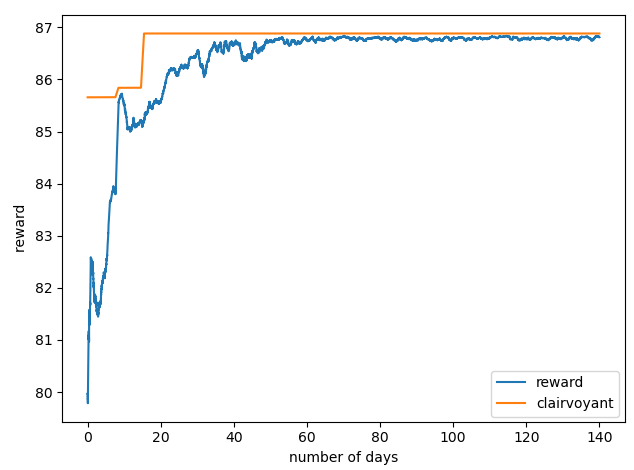
\includegraphics[width=0.9\textwidth]{../curves/results/context_generator_2000clicksperday_reward}}
\makebox[\textwidth][c]{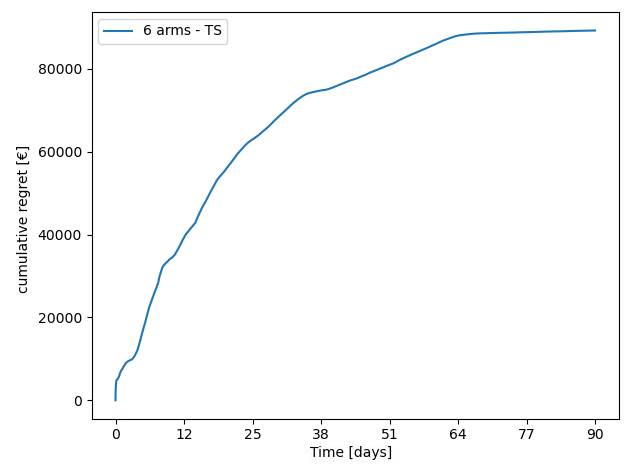
\includegraphics[width=0.9\textwidth]{../curves/results/context_generator_2000clicksperday_regret}}\\\\\\\\
By watching the clairvoyant plot, it is clear that the splits happened two times (expected since there are three class of users), the first one in the first week of the experiment, and the second one on the second week. \\The reward deviates more from the clairvoyant in the initial weeks, when the splits still need to happen and influence the computations of the following weeks, and later converges to the clairvoyant, once the shift to the splitted scenario occurs. \\Complementary, the cumulative regret graph shows an exponential and more substantial growth in the first weeks, and later settles after the splits have influenced the reward.